\section*{Empirical Specification}

In this section, I discuss the empirical framework used to estimate the implicit prices of housing attributes through a hedonic price model. I begin by describing the source and structure of the data, followed by the construction of a representative set of structural and neighborhood characteristics relevant to the valuation of residential properties. Next, I outline the rationale for geographically stratifying the analysis to account for spatial heterogeneity in housing markets. Finally, I review the core assumptions of the method of least squares and explain how model coefficients are interpreted within the log-linear specification.

\subsection*{Data Source and Structure}

The empirical analysis is based on a dataset of publicly available records from the Zillow website, focusing on residential properties marked as sold between January $2023$ and May $2025$.

The geographic scope of the study is limited to ZIP codes within the Orlando postal region, defined specifically as areas where the city name is listed as Orlando, FL. This definition ensures consistency in geographic coverage while capturing the urban and suburban variation within Orlando's housing market.

Extensive data cleaning and transformation procedures were conducted using Python. This process involved removing incomplete entries, standardizing formats, and engineering new variables relevant to housing structure, amenities, and location. The final dataset includes complete records on property sale price, sale date, structural features, and locational attributes, along with precise geographic identifiers such as city, county, street address, ZIP code, longitude, latitude. A detailed description of all variables, including their definitions and construction methods, is provided in the Appendix A.

\subsubsection*{Dependent Variable}

The dependent variable is the sale price of each residential property, recorded as the actual transaction price at the time of sale. This measure is of central importance in hedonic analysis, as it captures the revealed preferences of market participants. The observed sale price reflects the marginal willingness to pay for the full bundle of housing attributes associated with each property. Applying the natural logarithm of sale price during modeling is a practical transformation that helps address skewness and stabilize variance, improving the model’s interpretability and performance.

To ensure comparability over time, all prices were adjusted for inflation using the Consumer Price Index for All Urban Consumers \citep{bls:2024}. Prices were converted to constant May 2025 dollars using the formula:

\[
\text{Adjusted Price}_n = \frac{\text{Nominal Price}_i}{\text{CPI}_{t(n)} / \text{CPI}_{\text{May 2025}}}
\]

\noindent where $\text{CPI}_{t(n)}$ is the CPI for the month of sale of property $n$, and
$\text{CPI}_{\text{May 2025}}$ is the CPI for the base period.


\begin{figure}[H]
	\centering
	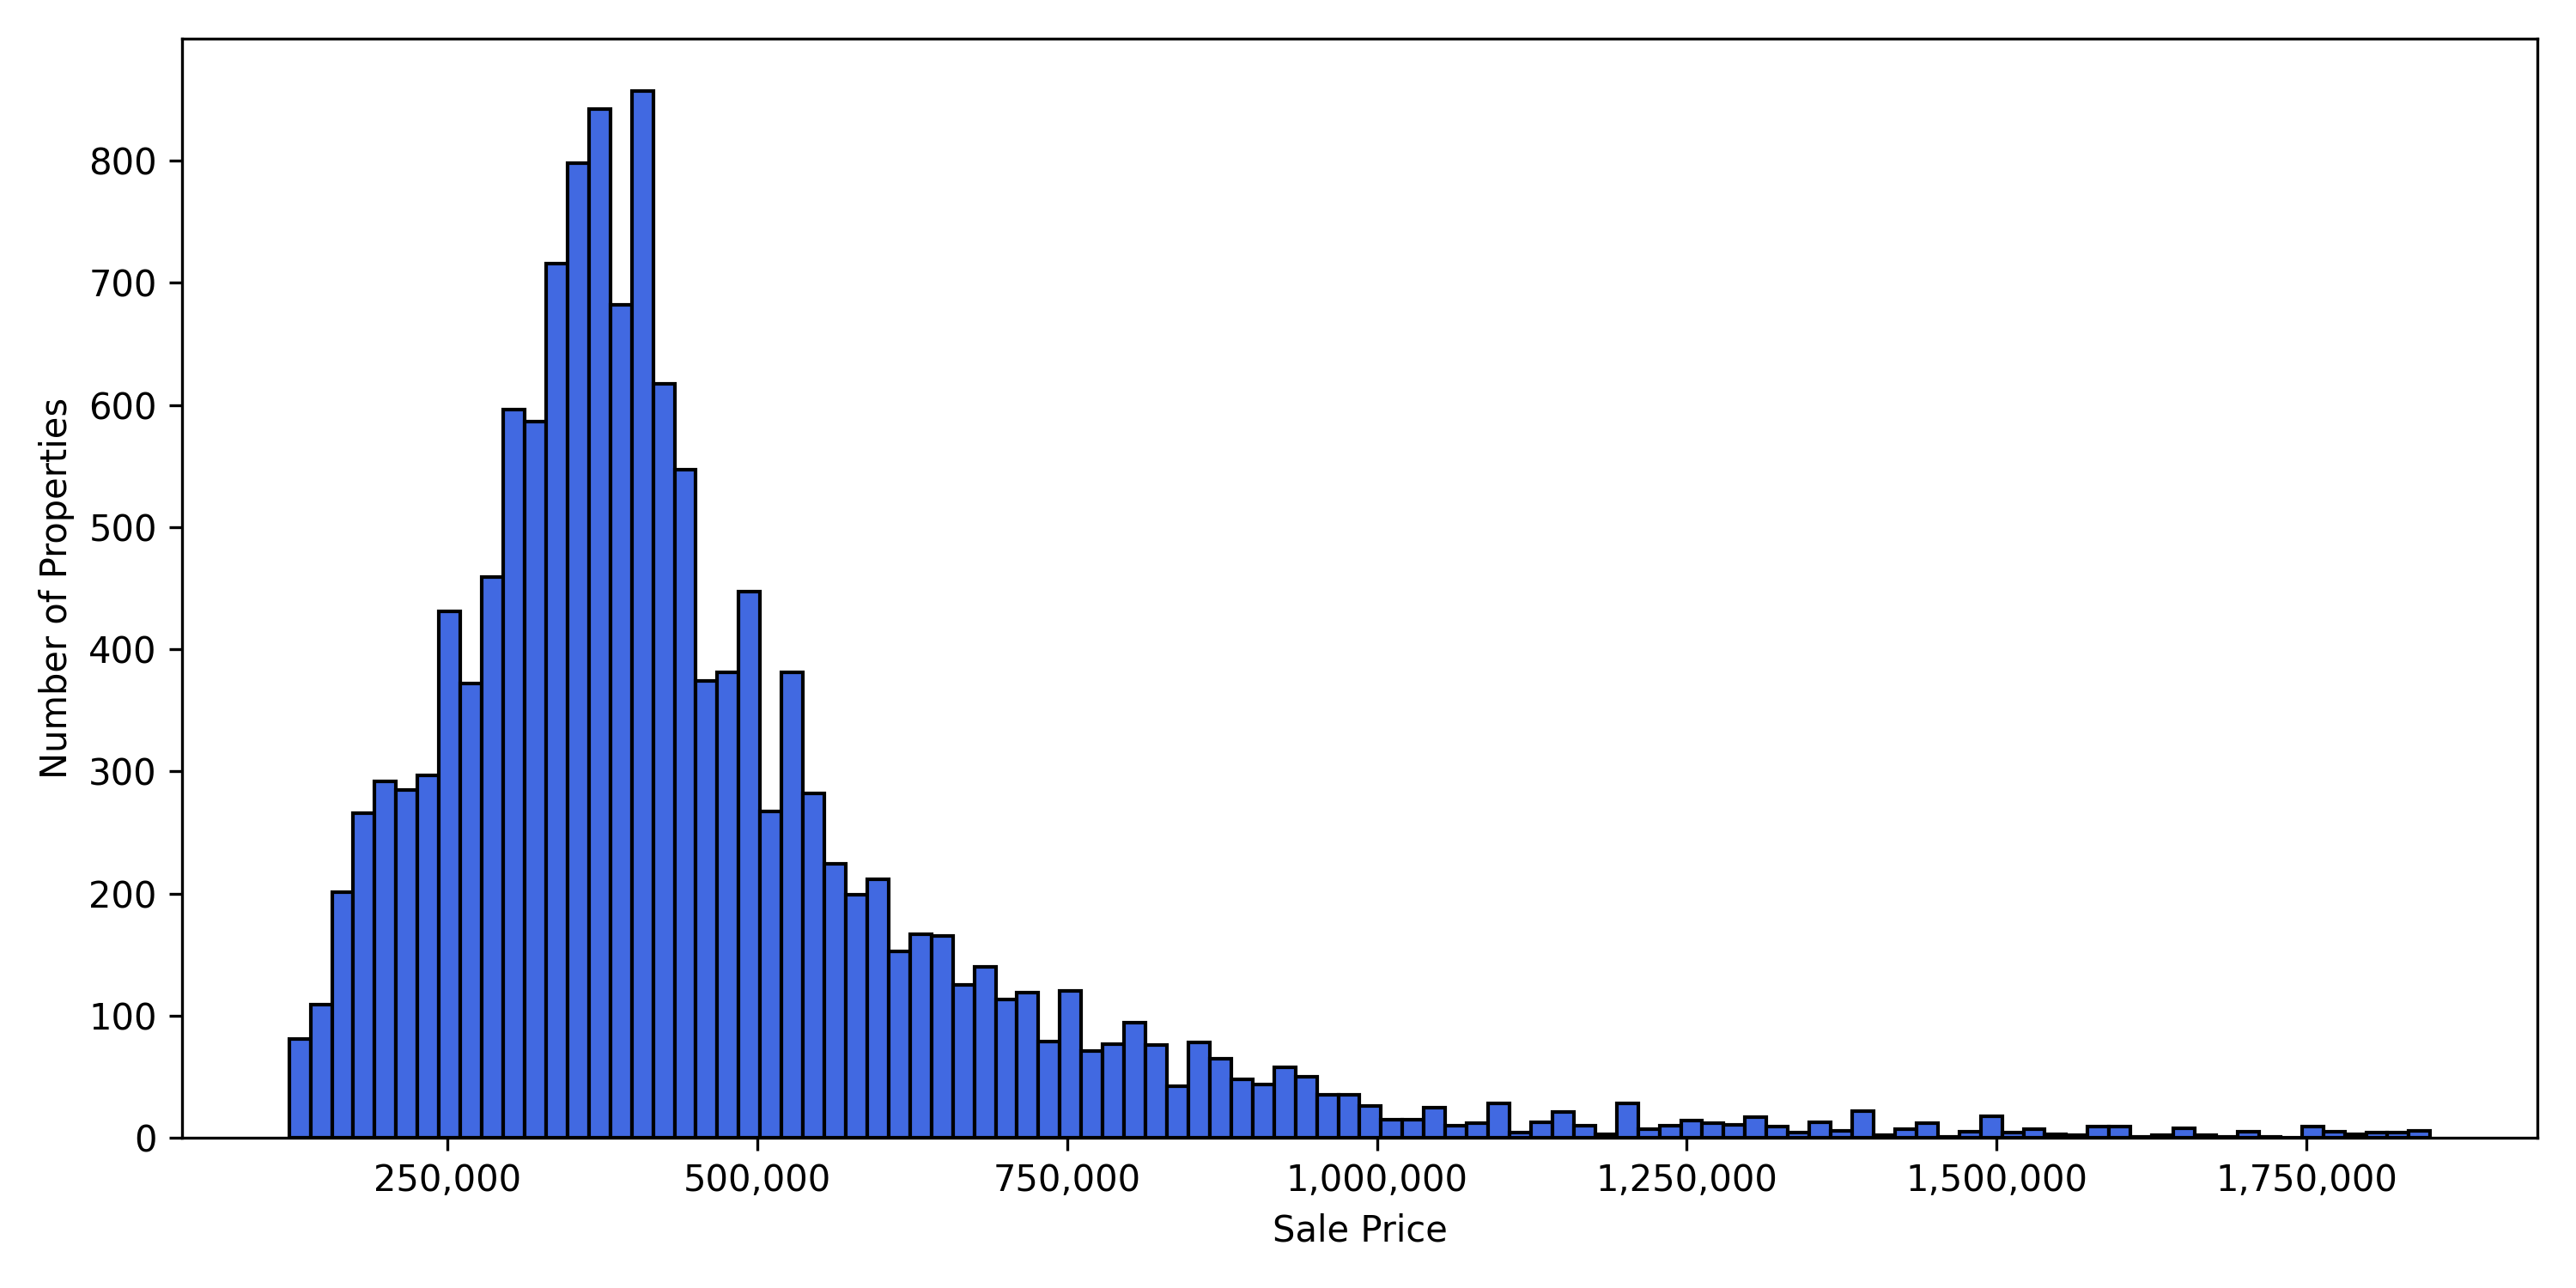
\includegraphics[width=0.9\textwidth]{Figures/sale_price_distribution.png}
    \caption{Distribution of Real Sale Prices in Orlando}
	\label{fig:1}
\end{figure}


\subsubsection*{Structural Characteristics}

Structural characteristics refer to the physical and functional features of each residential property. Variables capturing these characteristics include the type of home, the age of the property (measured as the difference between the sale date and the year built), total living area in square feet, the number of bedrooms and bathrooms, and the number of parking spaces. In addition, binary variables are used to capture the presence of a private pool and a garage.

\subsubsection*{Neighborhood Characteristics}

Neighborhood characteristics capture the broader context in which a property is located and play a key role in shaping buyer preferences beyond structural features. These include binary indicators for the presence of a homeowners’ association (HOA), gated community access, public parks, playgrounds, scenic views, and water views. Recreational amenities are summarized as a count of commonly listed features such as fitness centers, community pools, clubhouses, saunas, spas, and sports courts. Additional variables indicate whether a property is situated outside flood-risk zones, within the official boundaries of the City of Orlando, or adjacent to greenbelt areas comprising natural or agricultural land surrounding urban development. The dataset also includes school-related variables capturing the distance to the nearest elementary, middle, and high schools, as well as their respective ratings based on the GreatSchools rating system.

To assess the effect of proximity to transportation infrastructure on home prices, Manhattan distances were calculated from each property to the nearest exit along I -- $4$, SR -- $408$, SR -- $417$, SR -- $528$, and Florida’s Turnpike. Using \texttt{OpenStreetMap} data retrieved via the \texttt{OSMnx} library, a drivable road network was constructed and filtered to include only major highways and junctions. A custom \texttt{Python} function matched each home to the closest relevant exit based on keyword-matched road names and projected coordinates, producing distance measures in miles (see Appendix B). To simplify the model and to avoid redundancy, only the minimum distance to any of the five highways was retained as the final proximity measure.

\begin{table}
\caption{Summary Statistics}
\label{tab:summary_stats}
\begin{tabular}{lrrrrr}
\toprule
 & mean & std & min & 50\% & max \\
\midrule
sale\_price & 469521.62 & 238104.81 & 123640.77 & 412540.16 & 1976832.37 \\
home\_type & 2.62 & 0.71 & 1.00 & 3.00 & 3.00 \\
age & 29.99 & 20.08 & 1.00 & 29.00 & 108.00 \\
living\_area & 1867.30 & 745.55 & 576.00 & 1682.00 & 5989.00 \\
bedrooms & 3.34 & 0.84 & 1.00 & 3.00 & 8.00 \\
bathrooms & 2.57 & 0.78 & 2.00 & 2.00 & 7.00 \\
avg\_distance\_to\_schools & 1.74 & 0.72 & 0.33 & 1.67 & 5.97 \\
avg\_schools\_rating & 5.21 & 1.43 & 2.67 & 5.00 & 8.33 \\
min\_distance\_highway & 1.73 & 1.18 & 0.04 & 1.48 & 9.27 \\
sqft\_per\_bedroom & 555.20 & 138.73 & 212.00 & 536.00 & 1610.67 \\
\bottomrule
\end{tabular}
\end{table}


\subsection*{Geographic Stratification and Modeling Considerations}

Housing markets are inherently heterogeneous, with both property prices and the implicit prices of individual attributes varying substantially not only between cities, but also across neighborhoods within the same metropolitan area. These variations reflect differences in local market conditions and supply constraints. Even within a single city such as Orlando, housing is not traded in a perfectly competitive market, and preferences can vary widely across subpopulations. From an econometric standpoint, this presents a significant challenge: many utility-relevant characteristics are either unobserved or difficult to quantify, introducing the risk of omitted variable bias and reducing the precision of estimated coefficients \citep{abelson:1979}.

Although the inclusion of a broad set of characteristics generally improves the explanatory power of predictive models, it also introduces practical econometric challenges. By focusing on smaller, more uniform geographic areas, the variability in certain attributes is naturally reduced, which helps address the problem of unobserved heterogeneity and allows for a more parsimonious model specification, thereby improving the stability and interpretability of the estimates.

Therefore, ZIP code data were consolidated into five distinct subregions of Orlando: Orlando Central, Orlando West, Orlando East, Orlando Southeast, and Orlando South. These subregions were defined based on the City of Orlando Commission District boundaries, which reflect administratively relevant, demographically cohesive, and geographically contiguous units. \citep{orangecounty2025}.



\subsection*{Interpretation of Coefficients}

Given the log-linear price function, the marginal implicit price for any individual attribute $z_{nk}$ is given by:

\[
\frac{\partial P_n}{\partial z_{nk}} = \beta_k \, P_n
\]

\noindent This expression indicates that the marginal contribution of a one-unit increase in attribute $z_{nk}$ is proportional to both the estimated coefficient $\beta_k$ and the property's price $P_n$. Because the dependent variable is in logarithmic form, the coefficient $\beta_k$ can be interpreted as the approximate proportional effect on price --- so that $\beta_k \cdot 100$ percent  is the percentage change in price resulting from a one-unit increase in $z_{nk}$, holding all other attributes constant.
